% chktex-file 3 chktex-file 9 chktex-file 12 chktex-file 17 chktex-file 18 chktex-file 36 chktex-file 40
\section*{Exercise 18}

Let $\{X_{t} \}$ be any stationary series with continuous spectral density $\mathit{f}$ such that $0 \leq f ( \lambda) \leq K$ and $f ( \pi) \neq0$.

Let $f_{n} ( \lambda)$ denote the spectral density of the differenced series $\{( 1-B )^{n} X_{t} \}$.
\begin{enumerate}[label=(\alph*)]
    \item  Express $f_{n} ( \lambda)$ in terms of $f_{n-1} ( \lambda)$ and hence evaluate $f_{n} ( \lambda)$.
    \item Show that $f_{n} ( \lambda) / f_{n} ( \pi) \to0$ as $n \to\infty$ for each $\lambda\in[ 0, \pi)$.
    \item What does (b) suggest regarding the behaviour of the sample-paths of $\{( 1 - B )^{n} X_{t} \}$ for large values of $n?$.
    \item Plot $\{( 1 - B )^{n} X_{t} \}$ for $n=1$, 2, 3 and $4 ~$, where $X_{t}, \, t=1, \, \ldots,$ 100 are the
    Wolfer sunspot numbers (Example 1.1.S). Do the realizations exhibit the behavior expected from (c)? Notice the dependence of the sample variance on the order of differencing. (The graphs and the sample variances can be
    found using the program PEST.)
\end{enumerate}


\subsection*{Solution Part (a)}

Using \textbf{Theorem 4.4.1} we obtain that if $Y_t = (1-B) X_t$, then the spectral distribution of $Y$ is

\[ \everymath{\displaystyle}
\arraycolsep=1.8pt\def\arraystretch{2.5}
\begin{array}{rcl}
    F_Y(\lambda) & = & \int_{-\pi}^{\lambda} \left| 1 - e^{-it} \right|^2 f_X(t) dt\\
    & = & \int_{-\pi}^{\lambda} (1-e^{-it})\ol{(1-e^{-it})}f_X(t) dt\\
    & = & \int_{-\pi}^{\lambda} (1-e^{-it})(1-e^{it})f_X(t) dt\\
    & = & \int_{-\pi}^{\lambda} (2-(e^{-it} + e^{it})) f_X(t) dt\\
    & = & \int_{-\pi}^{\lambda} (2-2\cos(t)) f_X(t) dt\\
\end{array} \]
Thus, by the Fundamental Theorem of Calculus
\[ f_(Y)(\lambda) = (2-2\cos(\lambda)) f_{X}(\lambda), \]
and therefore,
\[ f_n(\lambda) = 2^n (1-\cos(\lambda))^n f_X(\lambda). \]

\subsection*{Solution Part (b)}

From the previous result, it follows that since $\lambda \in [0,\pi)$, $(1-\cos(\lambda)) < 2$, and thus,
\[ \frac{f_n(\lambda)}{f_n(\pi)} = \frac{2^n (1-\cos(\lambda))^n}{2^n (1-(-1))^2} \frac{f_X(\lambda)}{f_X(\pi)} = \frac{(1-\cos(\lambda))^n}{2^n} \frac{f_X(\lambda)}{f_X(\pi)} \to 0.\]

\subsection*{Solution Part (c)}

The function $f_n$ is maximized at $\lambda = \pi$ with $f_n(\pi) = O(4^n)$ while at any other frequency, $f_n(\lambda) = O(2^n (1-\cos(\lambda))^n)$, and $f_n(0) = 0$ minimizes the function. In fact, according to\textbf{ Proposition 4.5.3} $0 \leq \Var((I-B)^n X_t) \leq 2\pi 4^n f_X(\pi)$. So the values of $\nabla^n X_t$ might get exponentially larger and the period exponentially shorter when $n \to \infty$.

\subsection*{Solution Part (d)}

In order to plot the diffs of the sunspot numbers' sample we use the following Python code

\begin{minted}{python}
    import numpy as np
    import matplotlib.pyplot as plt
\end{minted}

\begin{minted}{python}
    X = np.array([
        101, 82, 66, 35, 31, 7, 20, 92, 154, 125,
        85, 68, 38, 23, 10, 24, 83, 132, 131, 118,
        90, 67, 60, 47, 41, 21, 16, 6, 4, 7, 
        14, 34, 45, 43, 48, 42, 28, 10, 8, 2,
        0, 1, 5, 12, 14, 35, 46, 41, 30, 24,
        16, 7, 4, 2, 8, 17, 36, 50, 62, 67,
        71, 48, 28, 8, 13, 57, 122, 138, 103, 86,
        63, 37, 24, 11, 15, 40, 62, 98, 124, 96,
        66, 64, 54, 39, 21, 7, 4, 23, 55, 94,
        96, 77, 59, 44, 47, 30, 16, 7, 37, 74
    ])
    years = np.arange(1770,1870)
    plt.plot(X)
\end{minted}
\begin{figure}[H]
    \centering
    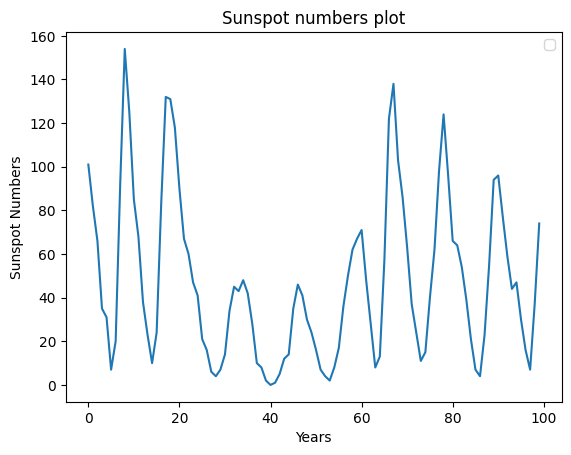
\includegraphics[width=0.85\textwidth]{../pictures/image6.png}
\end{figure}

\begin{minted}{python}
    from functools import reduce
    I = lambda X : X[1:]
    B = lambda X : X[:-1]

    for n in range(1,5):
        years_reduced = reduce(lambda x, _: I(x), range(n), years)
        I_minus_B_n_times = reduce(lambda x, _: I(x)-B(x), range(n), X)

        plt.figure()
        plt.plot(years_reduced, I_minus_B_n_times, label=f'n={n}')
        plt.xlabel("Years")
        plt.ylabel(rf"$\nabla^{{{n}}} X$")
        plt.title(f"Plot for $n$={n}")
        plt.legend()
        plt.show()
\end{minted}


\begin{figure}[H]
    \centering
    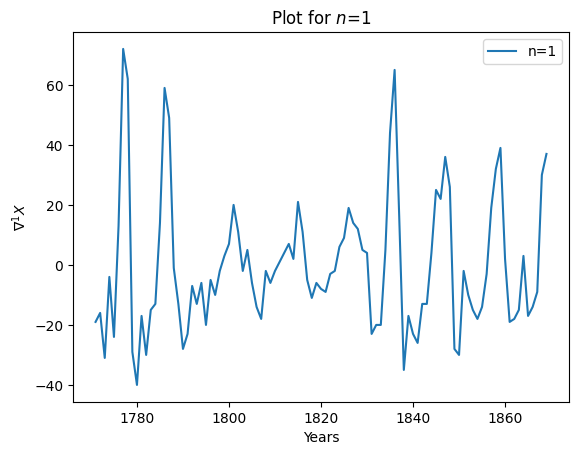
\includegraphics[width=0.45\textwidth]{../pictures/image2.png}
    \hfill
    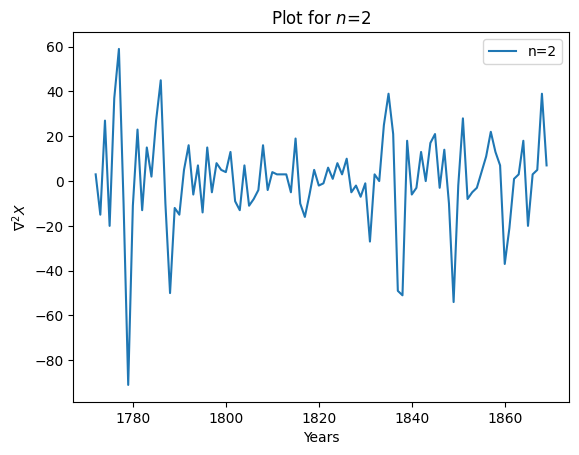
\includegraphics[width=0.45\textwidth]{../pictures/image3.png}
\end{figure}

\begin{figure}[H]
    \centering
    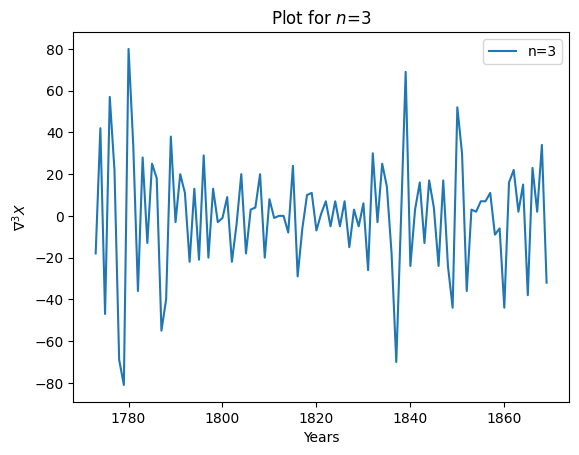
\includegraphics[width=0.45\textwidth]{../pictures/image4.png}
    \hfill
    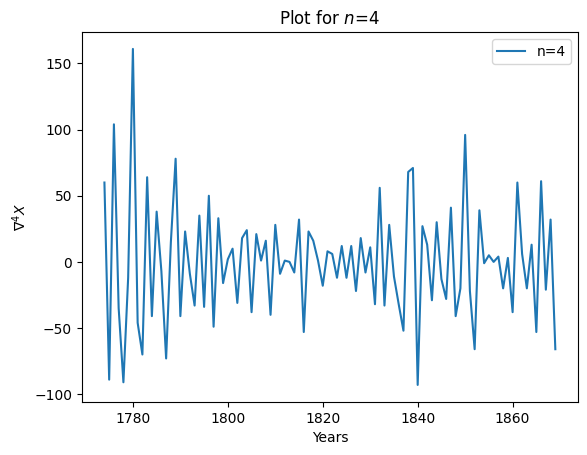
\includegraphics[width=0.45\textwidth]{../pictures/image5.png}
\end{figure}

Now, we'll see that the sample variance of $(I-B)^n X$ increases exponentially with the following code

\begin{minted}{python}
    variance = []
    for n in range(1,50,1):
        I_minus_B_n_times = reduce(lambda x, _: I(x)-B(x), range(n), X)
        variance.append(np.var(I_minus_B_n_times, ddof=1))
    plt.plot(np.log(variance))
    plt.xlabel("$n$")
    plt.ylabel(rf"$\log \overline{{\text{{Var}}}}(\nabla^n X)$")
    plt.title(rf"$n$ vs Sample variance of $\nabla^n X$")
    plt.legend()
    plt.show()
\end{minted}

\begin{figure}[H]
    \centering
    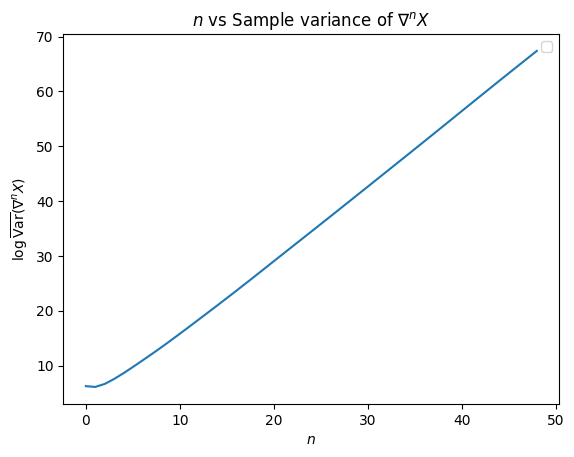
\includegraphics[width=0.85\textwidth]{../pictures/image7.png}
\end{figure}